\subsubsection*{NRM}

\paragraph{Overview}

Argo Node Resource Manager (NRM) is a daemon running on the compute
nodes. It centralizes node management activities such as job management,
resource management, and power management.

NRM interacts with both global resource management services (e.g., job
scheduler) and with application components and runtime services running on
the node. It acts as a control infrastructure to enable custom resource
management policies at the node level.  Applications can influence those
mechanisms, both directly (through explicit API calls used, e.g., to
request additional resources on the node) and indirectly (by having their
run-time behavior monitored by NRM).

\paragraph{Key Challenges}

Many ECP applications have a complex runtime structure, ranging from in
situ data analysis, through an ensemble of largely independent individual
subjobs, to arbitrarily complex workflow structures.  At the same time, HPC
hardware complexity increases as well, from deeper memory hierarchies to
heterogeneous compute resources and performance fluctuating based on
power/thermal constraints.

Even in the common case of each compute node being allocated exclusively to
a single job, managing available node resources can be a challenge.  If a
compute node is shared among multiple job components (a likely scenario
considering the reduced cost of data transfers), these components---if
allowed to freely share node resources---could interfere with one another,
resulting in suboptimal performance.  It is the NRM's job to rein in this
complexity by acting as a coarse-grained resource arbitrator.

\paragraph{Solution Strategy}

NRM uses \emph{slices} for resource management.  Physical resources on the
compute nodes are divided into separate partitions.  Slices can be used to
separate individual components of parallel workloads, in addition to
cordoning off system services; this physical separation ensures an improved
performance isolation between components.

Our slices can currently manage the CPU cores (hardware threads), the
memory and the kernel task scheduling class.  The physical
resources are partitioned primarily by using the \texttt{cgroups} mechanism
of the Linux kernel.  Work is under way to extend the management to 
the partitioning of last-level CPU cache using Intel's Cache Allocation
Technology.

The NRM daemon maps slices to the node's hardware topology, arbitrating
resources between applications and runtime services. Resources can be
dynamically reconfigured at run time; interfaces are provided for use from
applications and from global services.

\begin{wrapfigure}[10]{r}{.18\textwidth}
\vspace{-12pt}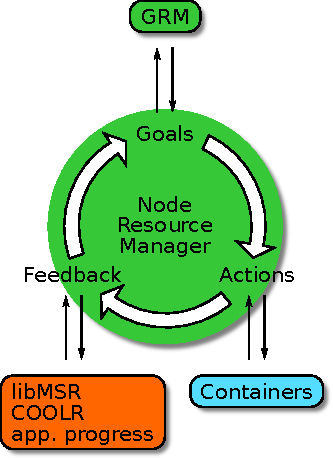
\includegraphics[width=.18\textwidth]{projects/2.3.1-PMR/2.3.1.19-Argo-PowerSteering/nrm-loop}
\end{wrapfigure}
The NRM daemon also manages power at the node level.  As depicted in the
figure on the right, it works in a closed control loop, obtaining goals
(power limit) from the global services (GRM), acting on application
workloads launched within slices by, for example, adjusting the CPU
\emph{p-states} or changing the power cap via the Intel \emph{RAPL}
mechanism, and getting feedback through the monitoring of hardware sensors
measuring, for example, power draw, temperature, fan speed, and frequency.

We provide a simple API that application processes can use to periodically
update the NRM on their progress.  This gives NRM reliable feedback on the
efficacy of its power policies, and it can also be used for a more robust
identification of the critical path, rather than relying on heuristics
based on performance counters.

\paragraph{Recent Progress}

%We developed an API between Node Power and Node Resource Manager (NRM),
%which in turn allows Global Resource Manager (GRM) to control and monitor
%power and other node-local resources.  Additionally, we studied the effect
%of power capping on different applications using the NodePower API and
%developed power regression models required for a demand-response policy.

%We developed the first version of the unified Node Resource Manager.  The
%NRM provides high level of control over node resources, including initial
%allocation at job launch and dynamic reallocation at the request of the
%application and other services.  The initial set of managed resources
%includes CPU cores and memory; they can be allocated to application
%components via a container abstraction, which is used to describe
%partitions of physical resources (to decrease interference), and more.  NRM
%integrates dynamic power control using COOLR and libMSR, and provides
%support for tracking and reporting of application progress.  Such
%functionality is needed by the BSP-oriented power policy, which we are
%currently evaluating and scaling up.  Work is also ongoing to support
%third-party container technologies such as Docker, Singularity, and
%Shifter.  At the job level, we enabled enclave-aware MPI facilities that
%can be used to create inter-communicators between MPI jobs launched in
%separate enclaves.

NRM has reached a pre-release quality level, with the source code of
version 0.1.0 being available on our website, and the documentation
provided on ReadTheDocs.  We have a custom CI pipeline in place that
ensures the stability via automated testing (we are making progress on
leveraging the ECP CI infrastructure as well).

We created the \texttt{libnrm} library that can be linked to applications
in order to provide reports on application progress to NRM.  We made an
initial effort of instrumenting a set of ECP application codes and
benchmarks: EXAALT, QMCPACK, ExaSMR, AMG, and Stream, with CANDLE underway.
This capability gives us insight into the effect of our resource management
policies on the run-time behavior of user codes.  Among other things, we
studied the power/performance tradeoffs of different applications under
varying power caps, as depicted in Fig.~\ref{fig:argo:nrm-results}.

\begin{figure}
\centering
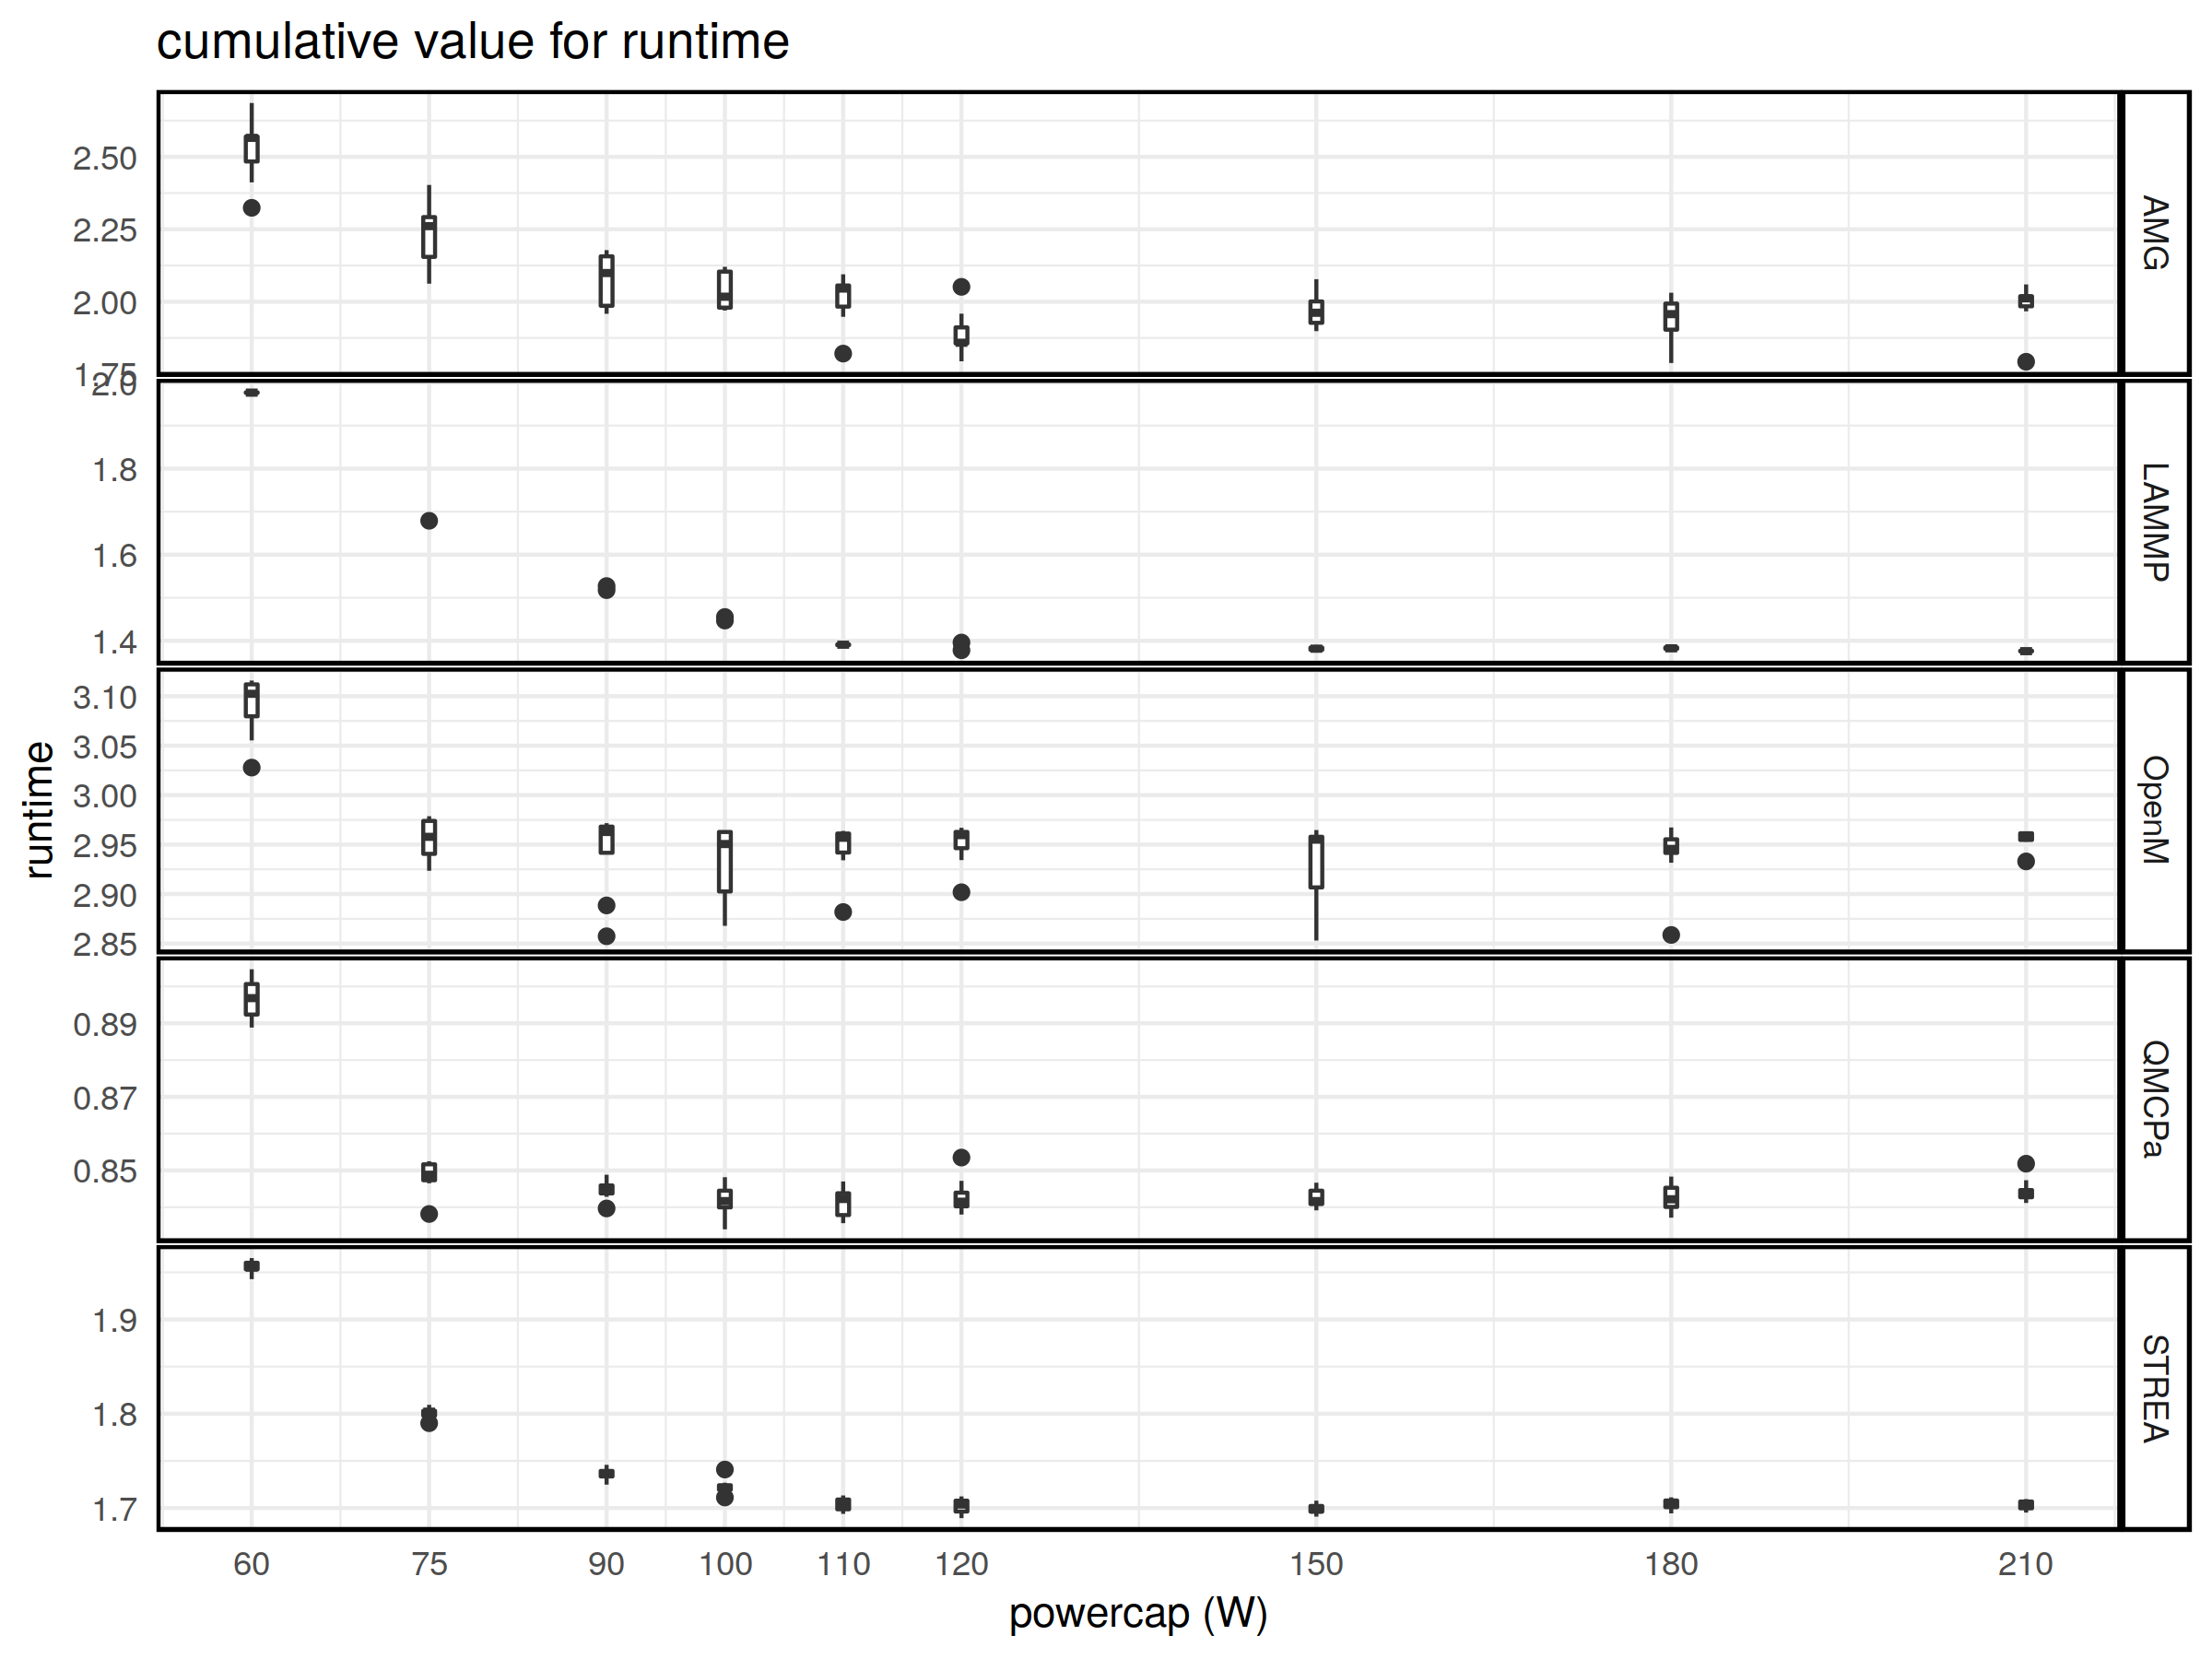
\includegraphics[width=.45\textwidth]{projects/2.3.1-PMR/2.3.1.19-Argo-PowerSteering/nrm-runtime}
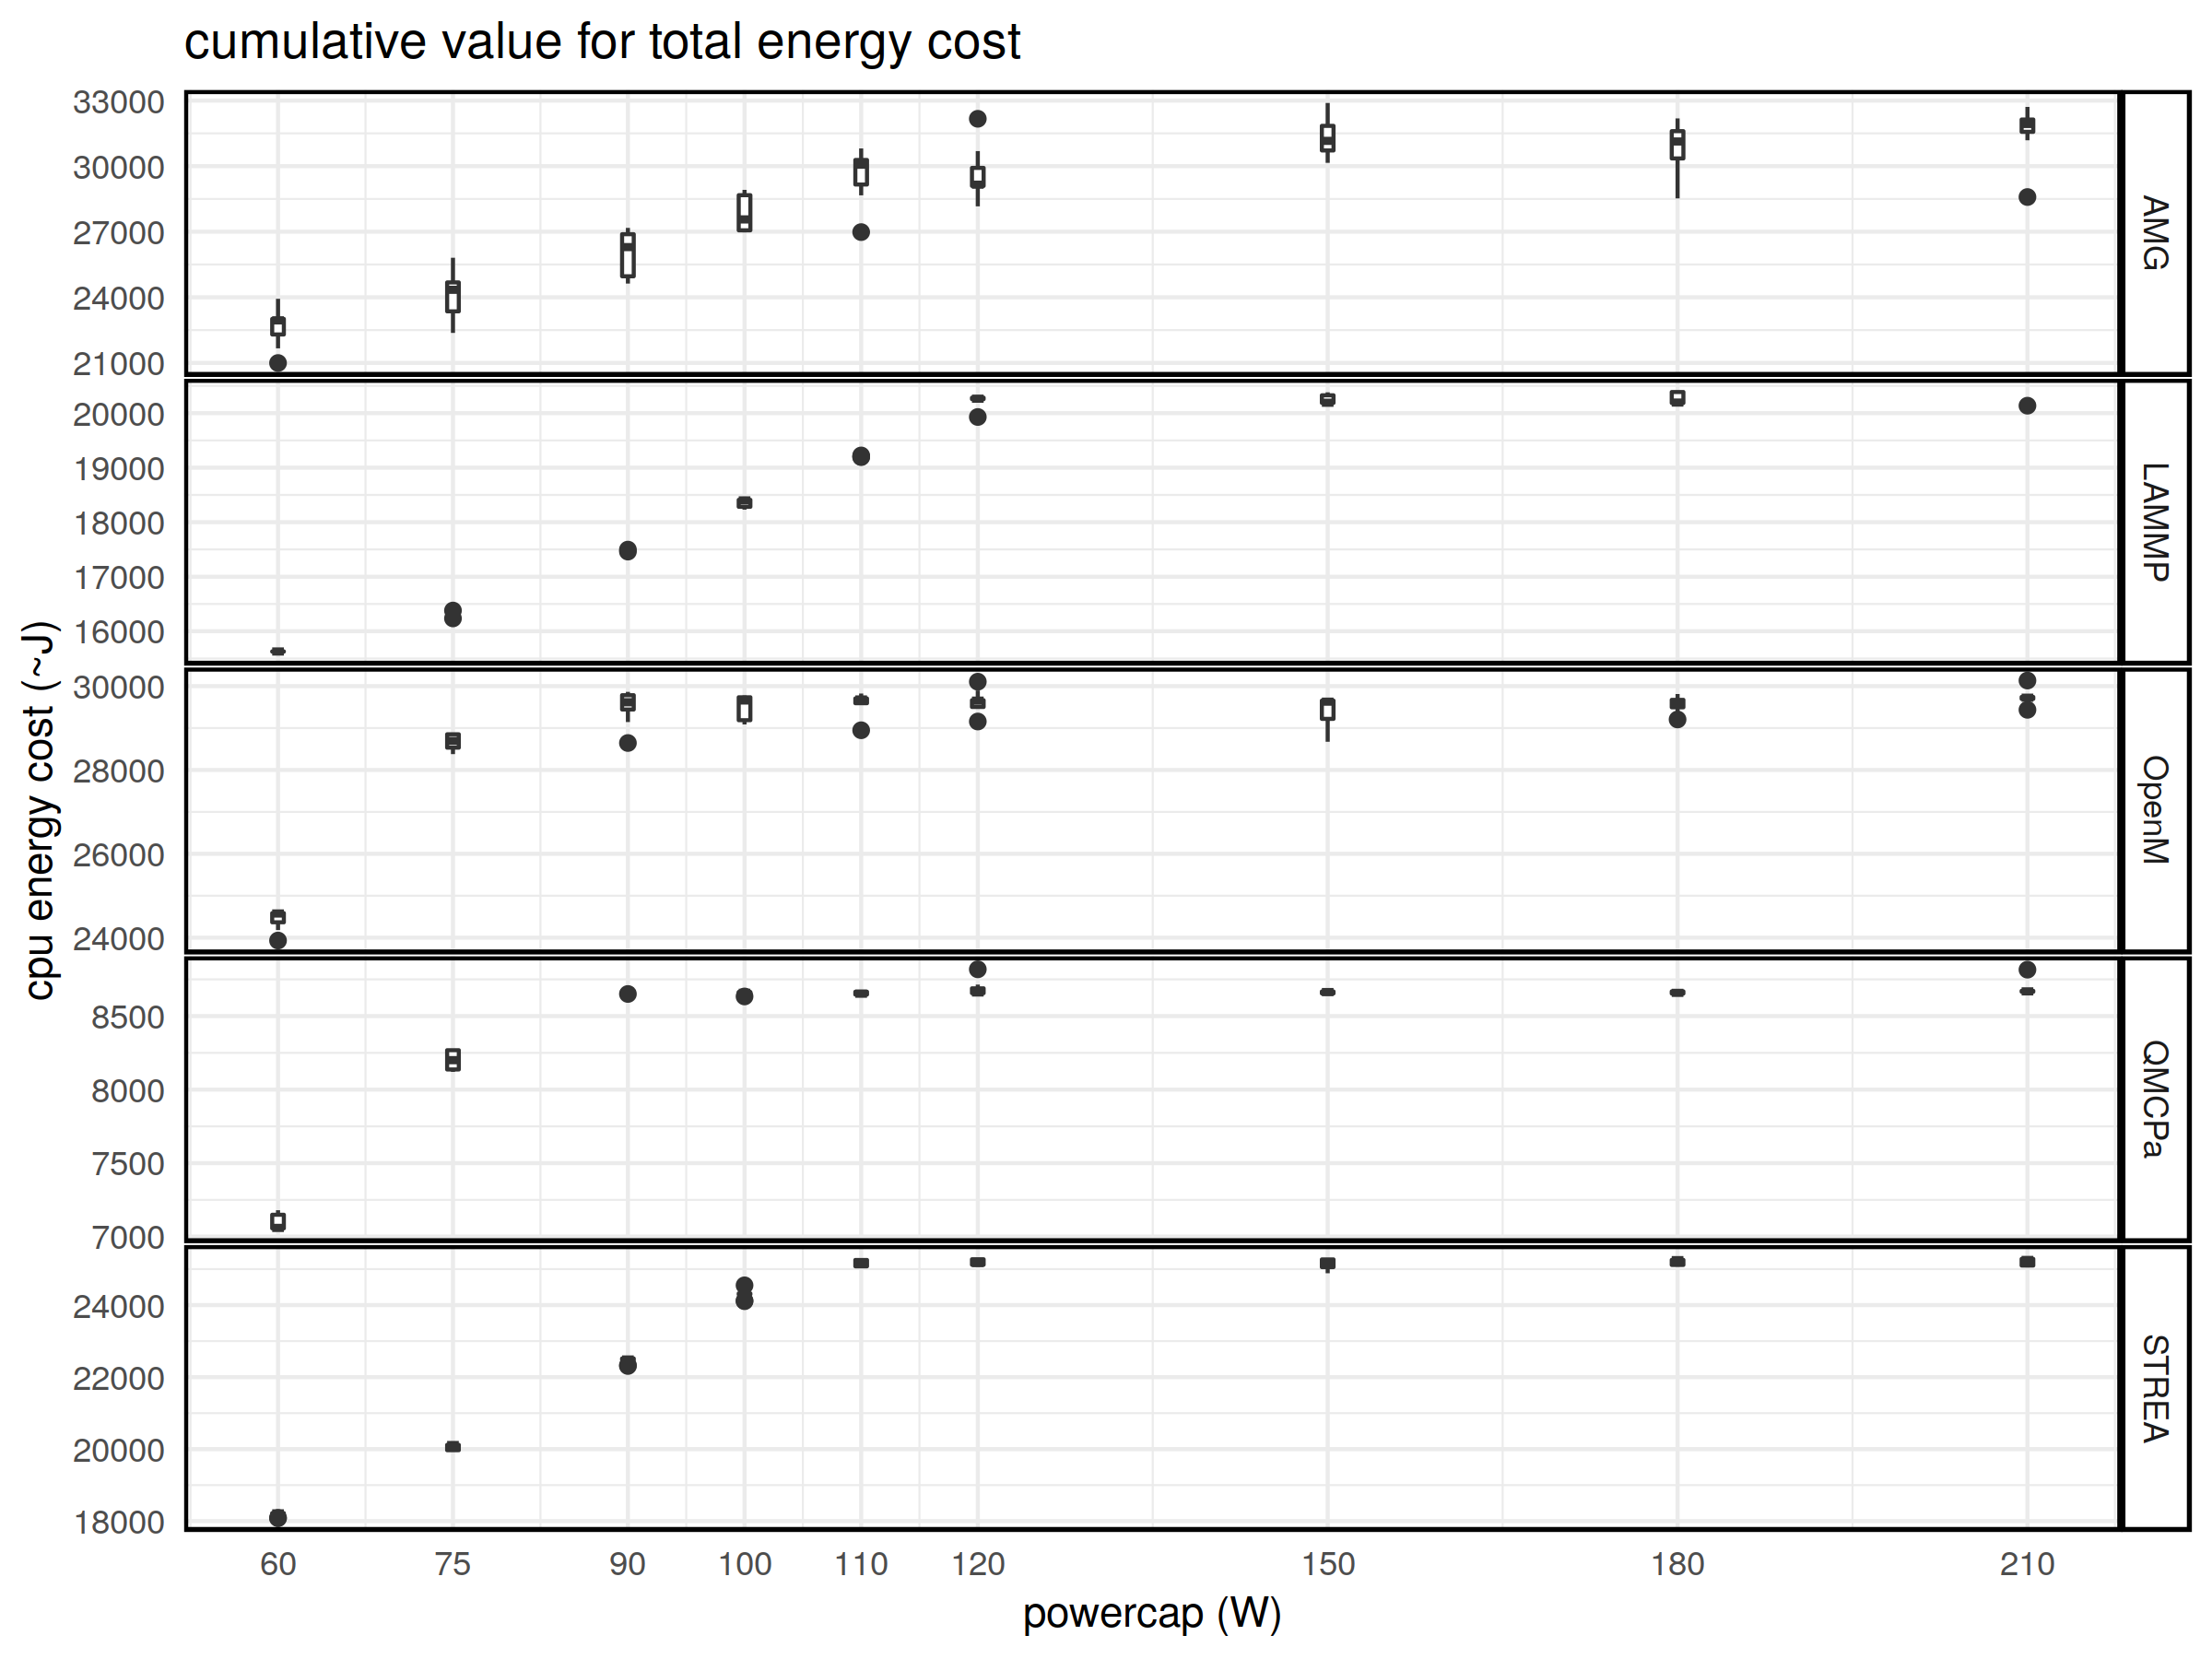
\includegraphics[width=.45\textwidth]{projects/2.3.1-PMR/2.3.1.19-Argo-PowerSteering/nrm-energy}
\caption{Cumulative run time and energy for different applications and
benchmarks running with a varying CPU power cap.}
\label{fig:argo:nrm-results}
\end{figure}

\paragraph{Next Steps}

We are working on expanding the set of ECP applications that are
instrumented to report their progress to NRM.  The reported data needs to
be propagated to the rest of the stack, and a resource management policy
needs to be created that takes advantage of this information.
%
We are expanding resource management to comprise of multiple policies, each
one optimized for a particular type of workloads, such as BSP, in-situ, and
workflows...  We are planning to provide a mechanism based on Machine
Learning techniques to automatically choose among the available policies.
%
We are also planning to expand interfaces for dynamic node resource control
in collaboration with applications, as well as adding an interface for
OpenMP codes akin to the PMPI functionality we already have.
%
We want to add support for standardized, OCI-based container runtimes by
adding a pass-through mechanism to our resource manager.
%
Finally, we are planning to expand the list of resources managed by NRM by
adding support for the partitioning of CPU caches and other vendor-specific
mechanisms.
